%% Submissions for peer-review must enable line-numbering 
%% using the lineno option in the \documentclass command.
%%
%% Preprints and camera-ready submissions do not need 
%% line numbers, and should have this option removed.
%%
%% Please note that the line numbering option requires
%% version 1.1 or newer of the wlpeerj.cls file.


%\documentclass[fleqn,10pt,lineno]{wlpeerj} % for journal submissions
\documentclass[fleqn,10pt]{wlpeerj} % for preprint submissions


%\newcommand{\rr}{${\mathcal{R}}$}
\usepackage{amssymb}
\usepackage{amsmath}
\usepackage{upgreek}
\usepackage[]{fontenc}
\usepackage{color}
\usepackage{bm}
\usepackage[english]{babel}
\usepackage{graphicx}
\usepackage{tikz}
\usetikzlibrary{positioning}
\usepackage{ifthen}
\usepackage{xstring}
\usepackage{afterpage}
%\usepackage[hidelinks]{hyperref}
\usepackage[colorlinks=true, allcolors=blue, pdfborder={0 0 0}]{hyperref}

\newcommand{\floor}[1]{\left \lfloor #1 \right \rfloor}
\newcommand{\round}[1]{\left \lfloor #1 \right \rceil }
\newcommand{\ceil}[1]{\left \lceil #1 \right \rceil }
\newcommand{\Fig}[1]{Fig.~\ref{#1}}
%\newcommand{\Fig}[1]{Figure~\ref{#1}}
\newcommand{\Figs}[1]{Figs.~\ref{#1}}
%\newcommand{\Figs}[1]{Figures~\ref{#1}}
\newcommand{\Sec}[1]{Section~\ref{#1}}
\newcommand{\Secs}[1]{Sections~\ref{#1}}
\newcommand{\Chap}[1]{Chapter~\ref{#1}}
\newcommand{\Chaps}[1]{Chapters~\ref{#1}}
\newcommand{\Tab}[1]{Table~\ref{#1}}
\newcommand{\Tabs}[1]{Tables~\ref{#1}}
\newcommand{\Eqn}[1]{Eqn.~\ref{#1}}
\newcommand{\Eqns}[1]{Eqns.~\ref{#1}}
\newcommand{\InEqn}[1]{Inequality~(\ref{#1})}
\newcommand{\InEqns}[1]{Inequalities~(\ref{#1})}
\newcommand{\Center}[1]{\textcolor{white}{.}\hfill#1\hfill\textcolor{white}{.}}
\newcommand{\ang}{$\textrm\AA$}
\newcommand{\new}[1]{#1}
\newcommand{\New}[1]{#1}
\newcommand{\n}[1]{#1}
\newcommand{\we}{I~}

\usepackage{xspace}

\newcommand{\pname}{\texttt{plotMAP}\xspace}
\newcommand{\code}[1]{\texttt{#1}\xspace}

\usepackage[cal=cm,scrscaled=1.05]{mathalfa} % This is for \mathcal{}, particularly \mathcal{R}
\DeclareMathAlphabet\mathbfcal{OMS}{cmsy}{b}{n} % for boldface mathcal: \mathbfcal{}
\newcommand{\rr}{$\mathcal{R}$\xspace}

\def\kt{k_{\rm B}T}


\def\beq{\begin{equation}}
\def\eeq{\end{equation}}
\def\bea{\begin{eqnarray}}
\def\eea{\end{eqnarray}}

\def\cal#1{\mathcal{#1}}
\def\eqq#1{Eq.~(\ref{#1})}
\def\eq#1{(\ref{#1})}
\def\av#1{\langle #1 \rangle}

\def\f#1{Fig.~\ref{#1}}
\def\ff#1{Figs.~\ref{#1}}

\def\s#1{Section~\ref{#1}}

\def\c#1{~\cite{#1}}


%\newcommand{\c}[1]{\citep{#1}}

\newcommand{\figdir}{./figures}

\title{A new and universal Ramachandran number $(\bm{\theta})$ as a reaction coordinate for protein backbone conformation}


\author[1,*]{Ranjan V. Mannige}
%\author[1]{Other Names TBD}
\affil[1]{~Multiscale Institute, Redwood City, CA, U.S.A.}
\affil[*]{~ranjanmannige@lbl.gov}

%\keywords{Ramachandran number, Multi-angle Picture, MAP, Protein structure}

\begin{abstract}
Proteins display complicated structures that often undergo numerous types of structural transformations. Without prior knowledge, it is often difficult to assess exactly where and how regions of a protein structure undergo structural transformation, which often makes it hard to survey new data, such as molecular dynamics trajectories or NMR-derived structural ensembles. Here, we present a suite of protein analysis tools -- \pname -- that utilize the Ramachandran number (\rr) in various formats in order to succinctly describe features of and dynamics within a new protein ensemble.
\end{abstract}

\begin{document}

\flushbottom
\maketitle
\thispagestyle{empty}

\section*{Introduction}

% Introduce the difficulty of describing protien structures (and their dynamics) in graphical form, especially for molecular dynamics.
Over almost half a century, protein simulation has matured as a field \citep{Levitt1976,Karplus2014,Levitt2014,Warshel2014,Nussinov2014}. However, even though the methods involved with simulation have come a long way \citep{Frenkel2002,Jorgensen2013,Hirst2014}, and even through the computational cost of simulating a protein keeps getting lower, our methods to appraise the progress of a protein has not changed much since the inception of this field. For example, how does one assess whether a protein simulation has reached equilibrium? Practioners of biomolecular simulation methods 



Persistant homollogy \cite{Cang2015}


The field of protein simulation has been maturing for the last available to a protein bacckbone is Many lower dimensional values exist that 
flexibility rigidity index \cite{Xia2013,Opron2014,Opron2015}

low RMSD to the crystal structure = low energy \cite{Nishikawa1972,Levitt1976,Levitt1983,Levitt1983a,Rasse1974,Ooi1978,Cohen1980,Maiorov1994}



Proteins are a class of biomolecules unparalleled in their functionality \citep{Berg2006}. A natural protein may be thought of as a linear chain of beads, with each bead being one of 20 naturally occurring amino acids. 
%Its exact sequence of amino acids (its primary sequence) dictates much about the final conformation fo a protein. E.g., a protein of a specific sequence may repeatedly fold into (or assume) a certain three-dimensional conformation \citep{Berg2006}. 
Proteins are important partially because of the structures that they access: the conformations (conformational ensemble) that a protein assumes determines the functions available to that protein. However, all proteins are dynamic: even stable proteins undergo long-range motions in its equilibrium state; i.e., they have substantial diversity in their conformational ensemble \citep{Mannige2014b}. Additionally, a number of proteins undergo conformational transitions, without which they may not properly function. Finally, some proteins -- intrinsically disordered proteins -- display massive disorder whose conformations dramatically change over time \citep{Uversky2003, Fink2005, Midic2009, Espinoza-Fonseca2009, Uversky2010, Tompa2011, Sibille2012, Kosol2013, Dunker2013, Geist2013, Baruah2015}, and whose characteristic structures are still not well-understood \citep{Beck2008}.

Large-scale changes in a protein occur due to changes in protein backbone conformations\footnote{Sidechain conformational changes alone, while correlated in space and time -- see \cite{DuBay2011} -- can not alone contribute to the change in a protein fold/conformation.}. 
\Fig{fig:intro}a represents atoms belonging to the backbone, which is represented by dark, filled bonds. \cite{Ramachandran1963} had recognized that the backbone conformational degrees of freedom available to an amino acid (residue) $i$ is almost completely described by only two dihedral angles: $\phi_i$ and $\psi_i$ [a third dihedral angle, $\omega_i$, is primarily planar at $180^\circ$; \cite{Pauling1951a,Pauling1951}]\footnote{See \Fig{fig:intro}a. For any amino acid $i$, $\phi_i$, $\psi_i$ and $\omega_i$ respectively involve the four atoms 
$\{\mathrm{C}_\mathrm{-1}, \mathrm{N}, \mathrm{C}\upalpha, \mathrm{C}\}$,
$\{\mathrm{N}, \mathrm{C}\upalpha, \mathrm{C}, \mathrm{N}_\mathrm{+1}\}$, and  
$\{\mathrm{C}\upalpha_\mathrm{-1}, \mathrm{C_{-1}}, \mathrm{N},\mathrm{C}\upalpha\}$.
The central bond involving $\omega_i$ describes the amide bond connecting residues $(i-1)$ and $i$. An alternative $\omega_i$ involves the connection between residues $i$ and $(i+1)$, where the four relevant atoms are $\{\mathrm{C}\upalpha, \mathrm{C}, \mathrm{N_{+1}},\mathrm{C}\upalpha_{+1}\}$.}. 
Today, protein structures described in context of two-dimensional $(\phi,\psi)$-space are called Ramachandran plots.

The Ramachandran plot is recognized as a powerful tool to obtain information about a protein backbone's conformation at a glance \citep{Berg2006,Alberts2002,Subramanian2001}. For example, particular regions within the Ramachandran plot indicate the presence of particular secondary structures such as the $\upalpha$-helix and $\upbeta$-sheet (see \Fig{fig:intro}b). Given this localization of secondary structure within the Ramachandran plot, it is also possible to interrogate the general features of a protein structure. E.g., given a discrete protein domain, it is possible to estimate a structure's secondary structure features %[and therefore it's general SCOP classification; \cite{Fox2014}] 
by the space that each residue occupies within the Ramachandran plot. Finally, certain parts of the Ramachandran plot are not permitted due to steric hindrance. Given this knowledge, it is possible to assess a newly solved protein structure's correctness or ``goodness'' by tracking the positions occupied by that structure in Ramachandran plot space \citep{Laskowski1993,Hooft1997,Laskowski2003}. 

\begin{figure}[t!]
\centering
\includegraphics[width=0.7\linewidth]{\figdir/fig1_intro.pdf}
\caption{\textbf{The Ramachandran number allows for a compact representation of protein backbone conformations}. Panel (a) represents a central amino acid (residue) along with its two neighbors. The structure of the backbone (black bonds) -- important in the overall structure of a protein -- is primarily described by the two dihedral angles $\phi$ and $\psi$; e.g., secondary structural elements of proteins fall in specific parts of the ($\phi$,$\psi$) or Ramachandran plot (b). %(to a lesser extent, the additonal dihedral angle $\omega$ may occupy one of two states -- \textit{cis} or \textit{trans}). 
A recent report \citep{MannigeKunduWhitelam2016} showed that ($\phi$,$\psi$)-pairs could be combined into a single order parameter -- the Ramachandran number (\rr) -- with relatively little loss of information. This means that descriptors of protein structure can be moved from two-dimensional Ramachandran plots to one-dimensional ramachandran lines (c). Assuming $N$ residues, while the number of variables are reduced from $2N$ to $N$ (from [$\phi_i$,$\psi_i$] $\to$ \rr$_i$, where $i\in{1,\cdots, N}$), the space in which the variables reside reduces from $N \times N$ to $N$ since $\phi_i$ and $\psi_i$ are not independent: only coupled together do they describe the structure of residue $i$. As a structural metric, the Ramachandran number (\rr)  is a lower dimensional descriptor when compared compared to ($\phi$,$\psi$).\label{fig:intro}} 
\end{figure}

While the Ramachandran plot has been useful as a descriptor of protein backbone conformation, it is not popularly used to assess structural dynamism and transitions (unless specific knowledge exists about whether a particular residue is believed to undergo a particular structural transition). This is because of the two-dimensionality of the plot: describing the behavior of every residue involves tracking its position in two-dimensional ($\phi$,$\psi$) space. Additionally, a third dimension $(\omega)$ also exists that further complicates things. Given enough residues, it would be impractical to track the position of each residue within a plot. Then comes time, where the positions of each point in the plot evolves. The possibility of picking out previously unseen conformational transitions and dynamism becomes a logistical impracticality.

However, it has recently been shown that the two values ($\phi$,$\psi$) may be conveniently combined into a single number -- the Ramachandran \textit{number} or $\mathcal{R}(\phi,\psi)$ -- with little loss of information \citep{MannigeKunduWhitelam2016}. 
In a previous report, detailed discussions were provided regarding the reasons behind and derivation of $\mathcal{R}$ \citep{MannigeKunduWhitelam2016}. After briefly reviewing the closed form of $\mathcal{R}$, this report discusses how $\mathcal{R}$ may be used to provide information about protein ensembles and trajectories. We call these pictograms ``MAPs'' (or simply ``maps''), an acronym for Multi-Angle Pictures. Finally, we introduce a software package -- \pname -- that can be used by to produce MAPs that describe the behavior of a protein backbone within user-inputted conformations, structural ensembles and trajectories. This package is presently available on GitHub (\url{https://github.com/ranjanmannige/plotmap.git}\textit{; preprint note: a pull request will need to be made initially to access as the repository is private}).

\section*{Need for compact protein structure descriptors}

Today, there is no single compact descriptor of protein structure. This impedes that na{\"i}ve or hypothesis-free exploration of new trajectories/ensembles\footnote{Of course, if prior knowledge (or hypothesis) existed that a structural transition occurred along a specific reaction coordinate -- say with the change in a particular atom-atom distance and or a particular dihedral angle -- then na{\"i}ve exploration would not be required. However, even in these situations, \pname would be important to provide structural fingerprints (see \Fig{fig:metrics}).}. For example, changes in protein trajectory is either comparitive or overly holistic: an example of a comparitive values is the root mean squared deviation in atomic position (compared, for example, to the the first conformation in the ensemble/trajectory);  an example of a holistic metric is the radius of gyration. While these metrics are heavily used by the molecular dynamics community, the change in these metrics over time or model number only provides a general sense that something in the structure is changing. These metrics, however, can not provide any more residue-level details than that. With protein dynamics undergoing a new rennissance -- especially due to intrinsically disordered proteins and allostery -- having hypothesis-agnostic metrics of protein structure has become even more relevant. Below, we will attempt to show that the Ramachandran number ($\mathcal{R}$), and the multi-angle picture, described below, is much more informational than prior ``na{\"i}ve metrics''.

\section*{Quick introduction to the Ramachandran Number $\bm{(\mathbfcal{R})}$}

The Ramachandran number is both an idea and an equation. Conceptually, the Ramachandran number ($\mathcal{R}$) is any closed form that collapses the dihedral angles $\phi$ and $\psi$ into one structurally meaningful number \citep{MannigeKunduWhitelam2016}. This paper will focus on the closed form presented in \cite{MannigeKunduWhitelam2016}. Assuming the bounds $[-180,180)$ for both dihedral angles, the previously described Ramachandran number takes the form 
\begin{equation}
\label{FirstRamachandran}
{\mathcal{R}}(\phi,\psi) \equiv  \frac{R_\mathbb{Z}(\phi,\psi)-R_{\mathbb{Z},\rm min}}{R_{\mathbb{Z},\rm max}-R_{\mathbb{Z},\rm min}}.
\end{equation}
Here, $R_\mathbb{Z}(\phi,\psi)$ is the un-normalized, integer-valued Ramachanran number. While further described in Methods-I (\Eqn{ramachandran3}), in short $R_\mathbb{Z}(\phi,\psi)$ is an indexing system whose value increases as one moves from the bottom-left to the top-right of the Ramachandran plot (see red arrows in \Fig{fig:intro}b), increasing over the plot in sweeps parallel to the negative-sloping diagonal (more discussion in Methods-I). 
%\begin{equation}
%R_\mathbb{Z}(\phi,\psi)  = \round{(\phi - \psi + \lambda)\sigma/\sqrt{2}} + \round{\sqrt{2} \lambda\sigma} \round{(\phi+\psi + \lambda)\sigma/\sqrt{2}}.\label{ramachandran3}
%\end{equation}
Finally, the minimum value $R_{\mathbb{Z},\rm min}\equiv R_\mathbb{Z}(-180,-180)$ and the maximum value $R_{\mathbb{Z},\rm max}\equiv R_\mathbb{Z}(180,180)$. Therefore, ${\mathcal{R}}(\phi,\psi)$ is normalized to range from 0 (bottom left) to 1 (top right), with intermediate values increasing from 0 along $-1/2$-sloping slices.

This report introduces an additional Ramachandran number -- the \textit{signed} Ramachandran number $\mathcal{R}_\textrm{S}$ -- which is identical to the original number in magnitude, but which changes sign from $+$ to $-$ as you approach $\mathcal{R}$ numbers that are to the right (or below) the positively sloped diagonal. I.e., 
\begin{equation}
\mathcal{R}_\textrm{S} = 
\begin{cases}
    \mathcal{R}         &\text{, if } \psi \geq \phi  \\
    \mathcal{R}\times-1 &\text{, if } \psi   <  \phi
\end{cases}\label{eqn:signed}
\end{equation}
For most proteins, very little of 
This metric is important for those glycine-rich peptides (and peptide-mimics such as peptoids) that both left and right regions of the Ramachandran plot; this is because, for such backbones, each $-1/2$-sloping slide of the Ramachandran plot may intersect more than one relevant region of the Ramachandran plot, which would put two structurally disparate regions within the Ramachandran plot close in $\mathcal{R}$-space. The signed Ramachandran plot $\mathcal{R}_\textrm{S}$ minimizes the probablity of this happening (see \Fig{fig_altr}). However, very few residues within structural databases occupy the right side of the Rmachandran plot ($3.5$\% ), which means that signed Ramachandran plots would only be useful in  special cases (and possibly for IDPs). For this reason, we will proceed below with a focus on the more relevant Ramachandran number $\mathcal{R}$.

It is useful to describe the reasons behind espousing the transition from ($\phi$,$\psi$) to $\mathcal{R}$ \citep{MannigeKunduWhitelam2016}: 1) as one transitions from low $\mathcal{R}$ to high $\mathcal{R}$, the backbone conformational properties smoothly transition; 2) $\mathcal{R}$ smoothly and monotonically increases with respect to both $\phi$ and $\psi$; and, importantly, 3) regions that describe particular secondary structures -- e.g., regions describing loops, $\upalpha$-helices and $\upbeta$-sheets -- are easily resolved in $\mathcal{R}$-space. This is made clear when comparing distributions of secondary structures within ($\phi$,$\psi$)-space (\Fig{fig:intro}b) and $\mathcal{R}$-space (\Fig{fig:intro}c). These points make  $\mathcal{R}$ a convenient and structurally meaningful descriptor of protein backbones.

%\begin{equation}
%{\mathcal{R}}(\phi,\psi) = \frac{\round{(\phi - \psi + \lambda)\sigma/\sqrt{2}} + \round{\sqrt{2} \lambda\sigma} \round{(\phi+\psi + \lambda)\sigma/\sqrt{2}} -\round{\lambda\sigma/\sqrt{2}}}{\round{\lambda\sigma\sqrt{2}}^2}.\label{ramachandran_expanded}
%\end{equation}

\section*{Reason to use the Ramachandran Number: it is stackable}

An important aspect of the Ramachandran number ($\mathcal{R}$) lies in its compactness compared to the traditional Ramachandran pair ($\phi,\psi$). Say we have an $N$-residue peptide. Then, switching from ($\phi,\psi$) to $\mathcal{R}$ \textit{appears} to only reduce the number of variables from $2N$ to $N$. However, ($\phi,\psi$) values are coupled, i.e., for any $N$-length peptide, any ordering of $[\phi_1,\phi_2,\ldots,\phi_N,\psi_1,\psi_2,\ldots,\psi_N]$ can not describe the structure, it is only \textit{pairs} -- $[(\phi_1,\psi_1),(\phi_2,\psi_2),\ldots,(\phi_N,\psi_N)]$ -- that can. Therefore, we must think of switching from ($\phi,\psi$) to $\mathcal{R}$ as a switch in structure space per residue from $N$ two-tuples $(\phi_i,\psi_i)$ that reside in $\phi\times\psi$ space to $N$ single-dimensional numbers ($\mathcal{R}_i$).

The value of this conversion is that the structure of a protein can be described in various one-dimensional arrays (per-structure ``Ramachandran codes'' or ``$\mathcal{R}$-codes''), which, when arranged vertically/columnarly, may then be \textit{stacked} side-by-side for visual/computational analysis. For example, the one-$\mathcal{R}$-to-one-residue mapping means that the entire residue-by-residue structure of a protein can be shown using a string of $\mathcal{R}_i$s (which would show regions of secondary structure and disorder, for starters). Additionally, an entire protein's backbone makeup can be shown as a histogram in $\mathcal{R}$-space (which may reveal a protein's topology). The power of this format lies not only in the capacity to distill complex structure into compact spaces, but in its capacity to display {\it many} complex structures in this format, side-by-side (stacking). The following proof-of-concept sub-section will show how stackability may be used in even a simpler but still important concept: understanding residue-specific backbone behavior.

\begin{figure*}
\centering
\includegraphics[width=\linewidth]{\figdir/ramachandran4.pdf}
\caption{\textbf{Ramachandran lines are stackable -- Part I.} 
Panel (a) shows the backbone behavior of an average residue (`*'), glycine (G) and proline (P) in $(\phi,\psi)$ -space, when these residues are present in globular proteins (see Methods). While these plots are useful (see Introduction), it is difficult to compare such plots. For example it is hard to pick out the change in the $\upalpha$-helial region of the proline plot, unless one manually draws a contour (brown line) that represents where the $\upalpha$-helix resides. However, when we convert Ramachandran plots to Ramachanran \textit{lines} [by converting $(\phi_i,\psi_i)\to\mathcal{R}_i$], we are able to conveniently ``stack'' Ramachandran lines calculated for each residue. Then, even visually, it is obvious that proline does not occupy the canonical $\upalpha$-helix region, which is not evident to an untrained eye in (a).\label{fig:peraa}}
~\vfill~
\includegraphics[width=\linewidth]{\figdir/motifs2.pdf}
\caption{\textbf{Ramachandran lines are stackable -- Part II.} Similar to \Fig{fig:peraa}c, the panel to the left in (a) represents the behavior of an amino acid `{\color{red}Y}' situated {\it before} a leucine (assuming that we are reading a sequence from the N terminal to the C terminal). The panel to the right similarly represents the behavior of specific amino acids situated before a proline. While residues preceeding a leucine behave similarly to their average behavior (\Fig{fig:peraa}a), most residues preceeding prolines appear to be enriched in structures that change `direction or backbone chirality (\rr$>0.5$). Panel (b) shows the behavior of individual amino acids when situated after each of the 20 amino acids. This graph shows a major benefit of side-by-side Ramachandran line ``stacking'': general trends become much more obvious. For example, it is evident that glycines and prolines dramatically modify the structure of an amino acid following it (compared to average behavior of amino acids in \Fig{fig:peraa}c). This trend is not as strong when considering amino acids that {\it follow} glycines or prolines (c). Such trends, while previously discovered [e.g., \cite{Gunasekaran1998,Ho2005}], would not be accessible when na{\"i}vely considering Ramachandran plots because one would require 400 ($20\times 20$) distinct Ramachandran plots per graph. Panel (d) facetiously represents 800 tiny Ramachandran plots, emphasizing the previous line.
\label{fig:motifs}}
\end{figure*}

\subsection*{Ramachandran lines are stackable: case study: residue-specific behavior.}

%Most structural biology textbooks discuss the behavior of the backbone of an average amino acid within the setting of a Ramachandran plot \citep{Berg2006,Alberts2002}. Often the average behavior is also compared to the behavior of specific amino acids such as glycine (CITE) and proline (CITE). 
This section illustrates the idea thatRamachandran plots [maps in $(\phi,\psi)$-space] are not easily comparible to one another, while Ramachanddran lines (maps in $\mathcal{R}$-space) are. \Fig{fig:peraa}a shows the backbone behavior, in $(\phi,\psi)$-space, of 1) an average amino acid (left), 2) glycine (middle), and 3) proline (right). Some features are immediately and easily discernable: glycine appears to be more symmetric across the negatively-sloping (dotted) diagonal (i.e., more structures with left-handed backbones are possible for glycines), while the $\upalpha_\textrm{D}$ region of the proline Ramachandran plot is completely unoccupied. However, it is not immediately apparant how dramatically different the rest of proline's Ramachandran plot is. 

At a glance, the proline backbone seems to occupy similar regions in the Ramachandran plot as backbones of average amino acids: both describe densities within the Ramachandran plot in the vicinity of the canonical $\upalpha$-helix (red/solid contour) and $\upbeta$-sheet (black/dashed contour). However, these two proline densities dominantly describe neither $\upalpha$-helices nor $\upbeta$-sheets. Prolines do not exist in regular $\upalpha$-helices\footnote{90\% of the time, when associated with $\upalpha$-helices, they are found in the first position of the helix, and other times they introduce ``kinks'' within an extended helix.}. Additionally, the density close to the $\upbeta$-sheet region of the backbone is does not actually conform to the $\upbeta$-sheet structure, but instead accounts for an extended helix called the polyproline II helix \citep{Adzhubei1993}\footnote{Prolines whose amide dihedral angles are in \textit{cis} conformation form polyproline I helices in generally the same region.}. While the Ramachandran plot would only reveal this type of nuance to someone with an unduely accurate understanding of secondary structure position. 

These differences are easily observable when stacking side-by-side Ramachandran lines for all amino acids (\Fig{fig:peraa}c). This type of simple comparison is next-to-impossible when comparing all of the 2D Ramachandran plots (\Fig{fig:peraa}b). Even when expiliclitely comparing the proline Ramachandran plot (\Fig{fig:peraa}a, bottom right) to the average Ramachandran plot (\Fig{fig:peraa}a, top), distinguishing between the two proline densities and the canonical $\upalpha$-helix and $\upbeta$-sheet regions of the Ramachandran plot is difficult unless a contour for both the regions are explicitely drawn. However, even glancing at \Fig{fig:peraa}c would reveal that proline backbones behave differently when compared to ther others.

While \Fig{fig:peraa} shows the convenience of comparing just 21 Ramachandran lines, \Fig{fig:motifs} shows how Ramachandran line ``stacking'' may be used to visually distill even larger structure spaces. In particular, \Fig{fig:motifs}b reveals that amino acids followed by prolines are ``different'' from those that follow any other amino acid in that more ``left-turning'' ($\mathcal{R} > 0.5$) backbone structures are visible. Residues \textit{preceeding} glycines and prolines do not display as much of a change from the norm (\Fig{fig:motifs}b). While this information is known \citep{Gunasekaran1998,Ho2005}, these discoveries may have been hastened with the use of Ramachandran lines.

\section*{The Python module PlotMAP}

\code{PlotMAP} is a software package written in Python that reads in protein structures and produces graphs based on the \rr number. These graphs depict the backbone structure in columnar fashion, one column ($\mathcal{R}$-code) per structure, so that structures are effectively stacked side by side for comparison. Since each column describes the entire backbone conformation as a collection of \rr numbers, and since, for every residue, \rr represents a compact form of $\phi$ and $\psi$ dihedral angles (\Fig{fig:intro}a), These graphs are called MAPs or multi-angle pictures (hense the name ``\pname''), because $\mathcal{R}$-codes provide a complete picture (map) of a protein backbone by displaying all backbone $(\phi,\psi)$ angles in compact form ($\mathcal{R}$). \Fig{fig:metrics} displays the various graphs that \pname is capable of producing for a single structure. However, its utility lies in displaying $\mathcal{R}$-codes for protein structure ensembles/trajectories.

\pname was designed to be used either as a stand alone tool or as a module, to be imported by other custom Python scripts. In its present form, \pname reads protein Protein Databank (PDB) formatted files \citep{Berman2000} and produces $\mathcal{R}$-codes that display either per-residue behavior of \rr or per-structure histogram distributions of the backboen in $\mathcal{R}$ space. 

The current implimentation of the package utilizes BioPython's \code{Bio.PDB} module \citep{Cock2009}. 


\begin{figure}
\centering
\includegraphics[width=\linewidth]{\figdir/fig2_metrics2.pdf}
\caption{For each structure inputted into \pname, the following graphs may be produced: traditional Ramachandran plot histograms (a), \rr histograms called (one form of an \rr-code) (b) and residue-by-residue \rr-codes (c). \rr-codes, unlike Ramachandran plots, occupies little space in the horizontal axis, and so they may be stacked side-by-side with other \rr-codes for visual analysis of structural changes (when comparing distinct conformations) and dynamism (when looking at equilibrium MD trajectories). The two protein structures used as examples are 1mba and 2acy and belong to two distinct SCOP classes \citep{Fox2014}.
\label{fig:metrics}}
\end{figure}

\section*{Methods - I. Arriving at the Ramachandran number $\bm{(\mathbfcal{R})}$}

To begin, we must first introduce the precursor to the Ramachandran number: the unnormalized Ramachandran number.

\subsection*{The unnormalized Ramachandran number $\bm{R_\mathbb{Z}}$.}
The Ramachandran number $\mathcal{R}$ is derived from the {\it unnormalized} Ramachandran number $R_\mathbb{Z}$ (`$\mathbb{Z}$' stands for integer), which is simply an integer-based indexing system \citep{MannigeKunduWhitelam2016}. Below is the previously discussed setup for calculating such numbers.

In order to satisfy historical notation \citep{Berg2006,Alberts2002,Laskowski1993,Laskowski2003}, we assume that Ramachandran plots range from $\phi,\psi \in [-180^\circ, \dots, 180^\circ)$. Given the periodicity of any dihedral angle, $\phi$ and $\psi$ values can be converted to fit this range\footnote{For example, an angle $\zeta$ can be wrapped within the range $[-180,180)$ using $\zeta' = - 180 + (\zeta + 180) \% (360)$, where $\%$ represents the modulus function.}. Accorrdingly, the unnormalized Ramachandran number \citep{MannigeKunduWhitelam2016} is
\begin{equation}
R_\mathbb{Z} \equiv R_\mathbb{Z}(\phi,\psi)  = \round{(\phi - \psi + \lambda)\sigma/\sqrt{2}} + \round{\sqrt{2} \lambda\sigma} \round{(\phi+\psi + \lambda)\sigma/\sqrt{2}}.
\label{ramachandran3}
\end{equation}
Here, $\round{x}$ rounds $x$ to the closest integer value, $\sigma$ is a scaling factor, discussed below, and $\lambda$ is the range of an angle in degrees (i.e., $\lambda=360$ and $\phi,\psi \in [-\lambda/2,\lambda/2]$). Effectively, this equation does the following. \textbf{1)} It divides up the Ramachandran plot into $(360^\circ \sigma^{1/\circ})^2$  squares, where $\sigma$ is a user-selected scaling factor that is measured in reciprocal degrees [see Fig.~8b in \cite{MannigeKunduWhitelam2016}]. \textbf{2)} It then assigns integer values to each square by setting the lowest integer value to the bottom left of the Ramachandran plot ($\phi=-180^\circ,\psi=-180^\circ$; green arrow in \Fig{fig:intro}b) and proceeding from the bottom left to the top right by iteratively slicing down -1/2 sloped lines and assigning increasing integer values to each square that one encounters. \textbf{3)} Finally, the equation assigns any $(\phi,\psi)$ pair within $\phi,\psi \in [-180,180]$ to the integer value ($R_\mathbb{Z}$) assigned to the divvied-up square that they it exists in. 

As long as $\sigma$ is kept large enough ($\sigma>10^{1/\circ}$ reciprocal degrees), original $(\phi,\psi)$ may be obtained with high accuracy from $R_\mathbb{Z}$ using the following equations:
\begin{align}
\tilde{\phi} &= \frac{1}{\sigma\sqrt{2}} \Big(\floor{R_\mathbb{Z} / \lambda'} + R_\mathbb{Z}\, \%\, \lambda' - \lambda' \Big), \label{backmap}\\
\tilde{\psi} &= \frac{1}{\sigma\sqrt{2}} \Big(\floor{R_\mathbb{Z} / \lambda'} - R_\mathbb{Z}\,  \%\,  \lambda' \Big).\label{backmap2}
\end{align}
Here, $\floor{x}$ indicates the largest integer smaller than $x$, $\%$ is the modulus function, and $\lambda' \equiv \round{\sqrt{2} \lambda\sigma}$ \citep{MannigeKunduWhitelam2016}. The error involved with the $R_\mathbb{Z}(\phi,\psi) \to (\phi,\psi)$ backmapping is much smaller than the expected error associated with the coordinates of structures in the Protein Databank [see Fig.~9 in \cite{MannigeKunduWhitelam2016}].

\subsection*{The Ramachandran number $\bm{\mathbfcal{R}}$.}
The unnormalized Ramachandran number $R_\mathbb{Z}$ (\Eqn{ramachandran3}) assumes arbitrary and conceptually ``meaningless'' integer values. However, the {\it normalized} Ramachandran number, or simply the Ramachandran number $\mathcal{R}$, assumes fractional values from 0 to 1 that are invariant of $\sigma$, and whose values are structurally meaningful. In particular, the normalization is performed as follows:
\begin{equation}
\label{ramachandran}
{\mathcal{R}}(\phi,\psi) \equiv  \frac{R_\mathbb{Z}(\phi,\psi)-R_{\mathbb{Z},\rm min}}{R_{\mathbb{Z},\rm max}-R_{\mathbb{Z},\rm min}}.
\end{equation}
Here $R_{\mathbb{Z},\rm min}\equiv R_{\mathbb{Z}}(-180,-180)$ and $R_{\mathbb{Z},\rm max}\equiv R_{\mathbb{Z}}(180,180)$.  When each residue within a peptide assumes the same backbone rotational state (i.e., when each residue describes on ($\phi,\psi$) pair and one $\mathcal{R}$), the following trends are evident: \textbf{1)} Peptides with $\mathcal{R} = 0, 0.5$ or $1$ are more extended (conversely, intermediary regions -- $\mathcal{R} \approx 0.28$ and $0.72$ -- describe the most collapsed peptides). \textbf{2)} $\mathcal{R}$ values lower than and greater than 0.5 respectively indicate right-handed and left-handed backbones (conversely, if two peptides describe repeating Ramachandran numbers that exactly equal $x$ and $1- x$, respectively, then the two peptide backbones are chiral opposites). \textbf{3)} $\upalpha$-helices and $\upbeta$-sheets respectively occupy average values of $\mathcal{R} \approx 0.36$ and $0.52$ (so, $\mathcal{R}$ $=0.36$ and $1-0.36$ respectively describe right- and left-handed $\upalpha$-helices). The next section elaborates on how $\mathcal{R}$ may be used to produce graphs that allow for the instantaneous and visual assimilation of complex protein conformations and conformational changes.

\subsection*{An alternative (signed) Ramachandran number $\bm{\mathbfcal{R}_\textrm{S}}$.} 
\label{altnumber}

As discussed above, the Ramachandran number depends on the iterative ``slicing'' across the ramachandran plot in lines that are parallel to the negative-sloping diagonal (dotted lines in \Fig{fig_altr}a). This means that structures that belong on the same negatively sloped line will have similar $\mathcal{R}$s, even if they are far away in $(\phi,\psi)$-space. This is not a problem with the secondary structures dominantly found in proteins, particularly because the backbones formed from natural amino acids with `L' or `pro-S' chirality)  dominantly occupy the ``left side'' of the plot ($\phi<0$; \Fig{fig_altr}a, top), a consequence of the chirality of the backbone $\alpha$-carbon \citep{Berg2006,Cintas2002} and steric hindrance between the backbone carbonyl and sidechain atoms (\cite{Branden1999}). Interestingly, switching the C$\alpha$'s chirality for every residue results in structures that exist on the ``other side'' of the plot, which a majority of its density at $\phi>0$; (\cite{Zacharias2013,Ho2003,Mannige2017a}). 

\begin{figure}[b!]
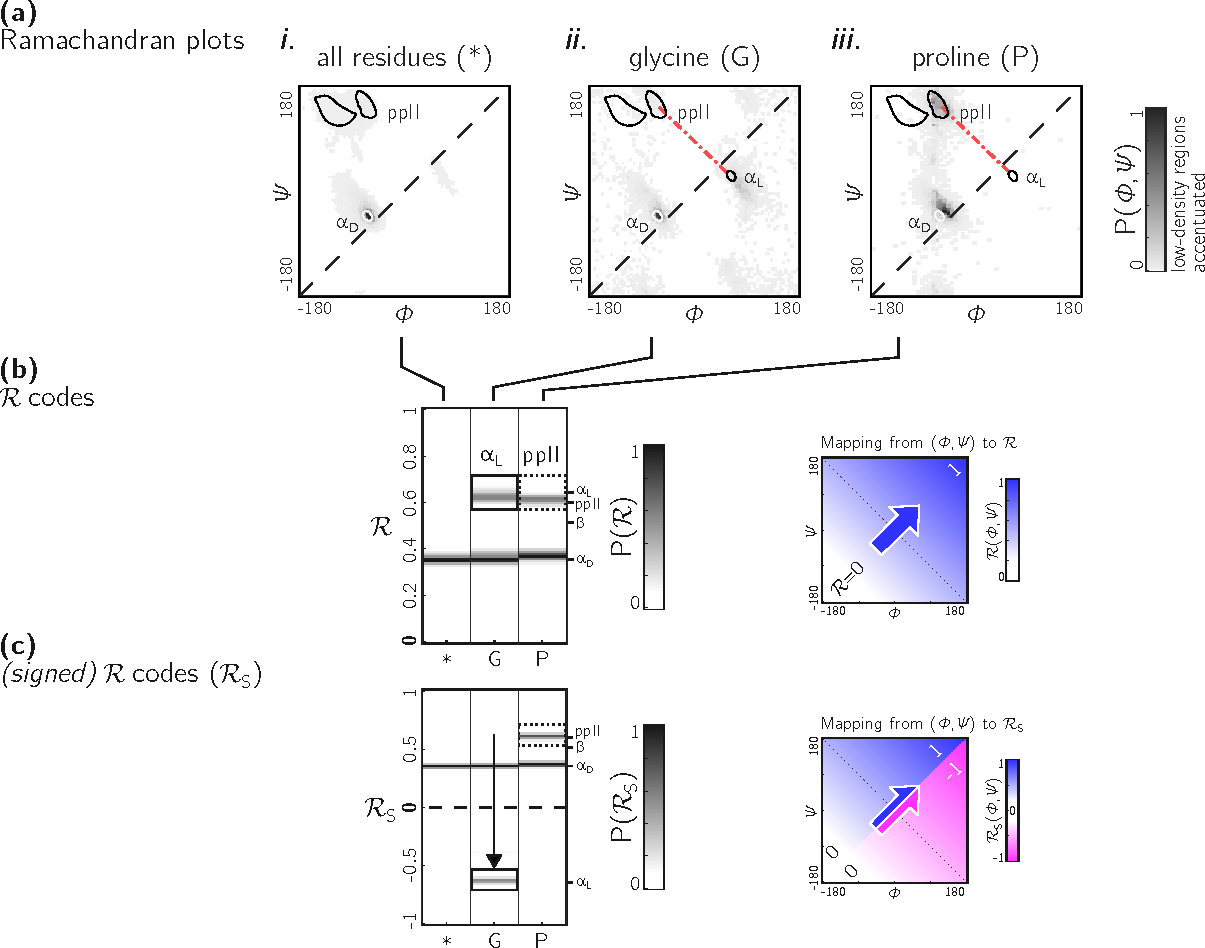
\includegraphics[width=\linewidth]{\figdir/signed4.pdf}
\caption{Ramachandran plots describing the backbone behavior of all residues, glycine, and proline are shown in (a). The polyproline II helical region (ppII; marked by a dotted square) and $\alpha_\textrm{L}$ region (solid square) roughly lie on the same negative-sloped line (solid, red). Because of this, their $\mathcal{R}$s are similar in value, and they are difficult to resolve using $\mathcal{R}$ (b). However, utilizing a {\it signed } Ramachandran number ($\mathcal{R}_\textrm{S}$; see \Eqn{eqn:signed}), we are able to easily resolve these values. Panels (c) and (e) show the mapping between the $(\phi,\psi)$ pair and $\mathcal{R}$ and $\mathcal{R}_\textrm{S}$, respectively. \label{fig_altr}}
\end{figure}

However, the $\alpha$-carbon of glycine is {\it not} chiral, and so is able to access both regions of the Ramachandran plot (\Fig{fig_altr}a, bottom left). This poses a problem for the Ramachandran number, as the secondary structure available almost exclusively to glycine -- the $\alpha_\textrm{L}$-helix (the chiral opposite of the $\alpha_\textrm{D}$- or simply $\alpha$-helix) -- lies on the same negative-sloping line that contains the polyproline II helix \citep{Chebrek2014} or ``ppII'' (\Fig{fig_altr}a, bottom; $\alpha_\textrm{L}$ and ppII regions are marked by solid and dotted squares in all panels; the negative-sloped line that connects these regions are drawn as dotted-dashed red lines in a). In \rr-space, both structures will have similar values, as is evident in the histograms (\rr-codes) in \Fig{fig_altr}b. \Fig{fig_altr}b represents the mapping between $(\phi,\psi)$ and $\mathcal{R}$, which shows the progression of $\mathcal{R}$ from $0$ and $1$.

Interestingly, a small change in assigning $\mathcal{R}$ values solves the problem of introducing backbones with achiral $\alpha$-carbons (e.g., glycine and peptoids). In particular, all $\mathcal{R}$s that exist to the below (or to the bottom-right) of the the positively sloped diagonal (dashed lines in \Fig{fig_altr}a) are multiplied by -1. In equation form, the Ramachandran number in \Eqn{ramachandran3} gets transformed by the following conditional:
\begin{equation}
\mathcal{R}_\textrm{S} = 
\begin{cases}
    \mathcal{R}\times-1 &\text{, if } \psi < \phi \\
    \mathcal{R}         &\text{, if } \psi \geq \phi 
\end{cases}\label{eqn:signed}
\end{equation}

\Fig{fig_altr}d shows how $\mathcal{R}_\textrm{S}$ resolves the regions associated with ppII and $\alpha_\textrm{L}$ by assigning negative $\mathcal{R}_\textrm{S}$ values to regions associated with the right side of the positive-sloped diagonal ($\alpha_\textrm{L}$). While $\mathcal{R}_\textrm{S}$ conveniently describes the backbone behavior of achiral $\alpha$-carbons, its utility in the protein world is limited, given that little of the ``negative region'' of the Ramachandran plot is regularly occupied. For this reason, we continue the rest of this discussion with the unsigned $\mathcal{R}$ in mind (although $\mathcal{R}_\textrm{S}$ may be thought of a simply the same as $\mathcal{R}$ -- since $\mathcal{R}=|\mathcal{R}_\textrm{S}|$ -- but with an additional piece of information).

\section*{Methods -- II. Data collection analysis}

\subsection*{Obtaining secondary structure statistics.}
\label{scop}

The panels in \Fig{fig:intro} and the secondary structural statistics within were borrowed from \cite{MannigeKunduWhitelam2016} (Figs.~3b,4). As described within \cite{MannigeKunduWhitelam2016}: $\alpha$-helices, $3_{10}$-helices and $\beta$-sheets were identified using the DSSP algorithm \citep{Zhao2005,Kabsch1983,Joosten2011} and sourced from protein structures within the 40\% non-redundant database provided by the Structural Classification of Proteins or SCOP (Release 2.03; \cite{Fox2014}). The polyproline II helix statistics were obtained from segments within 16,535 proteins annotated by PolyprOnline \citep{Chebrek2014} to contain three or more residues of the secondary structure.

\subsection*{Obtaining amino acid statistics.}
\label{scop}

Amino acid statistics (\Fig{fig:peraa}) and two-residue motif statistics (\Fig{fig:motifs}) were obtained from 13,760 proteins structural domains within the database hosted by the Structural Classification of Proteins or SCOPe (Release 2.06; \cite{Fox2014}) 
that contains proteins with no more than 40\% sequence identity (downloaded from 
\url{http://scop.berkeley.edu/downloads/pdbstyle/pdbstyle-sel-gs-bib-40-2.06.tgz}).\\
%\\ \verb+http://scop.berkeley.edu/downloads/pdbstyle/pdbstyle-sel-gs-bib-40-2.+\\
%\noindent\verb+06.tgz+). 
%Altogether, there were 13,760 proteins that were amenable to analysis from this database.

\subsection*{Obtaining trajectory statistics.}
\label{scop}

\textbf{Peptoid nanosheet.} The distribution for the $\Sigma$-sheet on a Ramachandran Plot (\Fig{fig1}c) and in an \rr-code (\Fig{fig_collage}, \Fig{fig_classes}b) were obtained from a 50 nanosecond interval of a molecular dynamics trajectory \citep{Mannige2015}. \Fig{fig_nanosheet}(b,c) describes a trajectory of the same system before and after the symmetry-enforcing backbone restraints were lifted. This process was part of a molecular dynamics equilibration step used in \cite{Mannige2015}.

The end-to-end distances for glycine peptides of 20 residues (\Fig{fig2}(a)) and 5 residues (\Fig{r_pathogen}(a)) were generated using the PeptideBuilder library\citep{Matthew2013} and analyzed using BioPython\citep{Cock2009}.


\section*{Acknowledgments}

RVM was supported by the Defense Threat Reduction Agency under contract no. IACRO-B0845281. RVM thanks Alana Canfield Mannige for her critique. This work was done at the Molecular Foundry at Lawrence Berkeley National Laboratory (LBNL), supported by the Office of Science, Office of Basic Energy Sciences, of the U.S. Department of Energy under Contract No. DE-AC02-05CH11231.

\bibliography{all}

\end{document}


\usepackage{grffile}
\usepackage{cancel}
%\usepackage{hyperref}
\usepackage{amssymb}
\usepackage{color}
\usepackage{amsmath}
\usepackage{bm}
\usepackage[english]{babel}
\usepackage{graphicx}
\usepackage{tikz}
\usepackage{ifthen}
\usepackage{xstring}
\usepackage{afterpage}
\usepackage{mathrsfs}
